\documentclass[border=10pt]{standalone}
\usepackage{pgfplots}
\pgfplotsset{compat=1.16}
\begin{document}
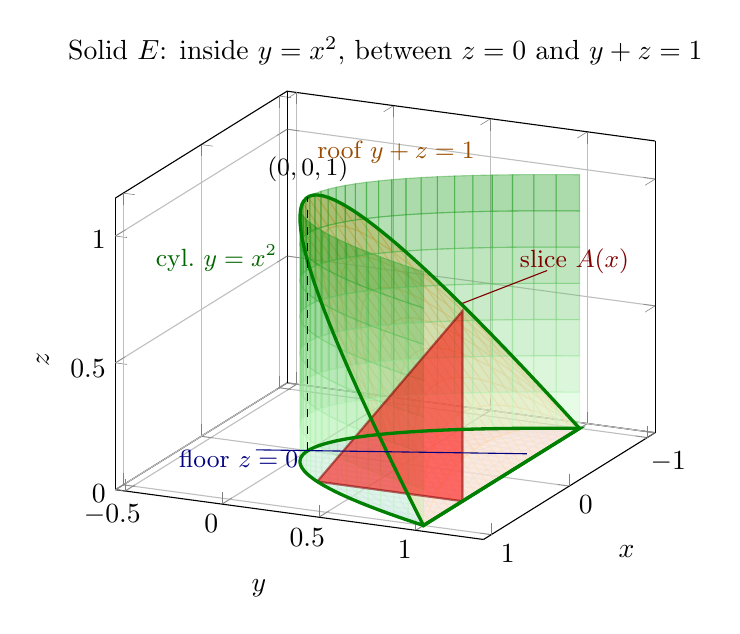
\begin{tikzpicture}
\begin{axis}[
    view={115}{22},
    xlabel={$x$}, ylabel={$y$}, zlabel={$z$},
    xmin=-1.1, xmax=1.1, ymin=-0.55, ymax=1.35, zmin=0, zmax=1.15,
    ztick={0,0.5,1}, grid=major,
    title={Solid $E$: inside $y=x^2$, between $z=0$ and $y+z=1$},
]
% Floor z = 0 over region R
\addplot3[surf, shader=flat, opacity=0.4,
    colormap={blues}{color=(blue!12) color=(blue!50)},
    domain=-1:1, samples=25, y domain=0:1, samples y=10]
    ({x}, {x^2 + (1 - x^2)*y}, {0});
% Roof plane z = 1 - y over region R
\addplot3[surf, shader=flat, opacity=0.5,
    colormap={oranges}{color=(orange!22) color=(orange!70)},
    domain=-1:1, samples=25, y domain=0:1, samples y=10]
    ({x}, {x^2 + (1 - x^2)*y}, {1 - x^2 - (1 - x^2)*y});
% Parabolic cylinder wall y = x^2
\addplot3[surf, shader=flat, opacity=0.35,
    colormap={greens}{color=(green!22) color=(green!55!black)},
    domain=-1:1, samples=40, y domain=0:1, samples y=8]
    ({x}, {x^2}, {y});
% Cross-sectional slice at x = 0.5 (right triangle)
\addplot3[fill=red, opacity=0.55, draw=red!50!black, thick]
    coordinates {(0.5,0.25,0) (0.5,1,0) (0.5,1,0.75) (0.5,0.25,0)};
% Parabola edges
\addplot3[green!50!black, very thick, domain=-1:1, samples=50] ({x}, {x^2}, {0});
\addplot3[green!50!black, very thick, domain=-1:1, samples=50] ({x}, {x^2}, {1-x^2});
% Vertical dashed segment at origin
\addplot3[dashed, black] coordinates {(0,0,0) (0,0,1)};
% Labels with leader lines
\node[anchor=east, text=orange!60!black] at (axis cs:-0.9,0.55,1.06) {\small roof $y+z=1$};
\node[anchor=west, text=blue!50!black] at (axis description cs:0.10,0.18) {\small floor $z=0$};
\draw[blue!50!black] (axis description cs:0.26,0.20) -- (axis cs:-0.45,0.95,0);
\node[anchor=east, text=red!50!black] at (axis description cs:0.97,0.62) {\small slice $A(x)$};
\draw[red!50!black] (axis description cs:0.80,0.60) -- (axis cs:0.5,1,0.78);
\node[anchor=east, text=green!40!black] at (axis cs:-0.85,-0.45,0.55) {\small cyl.\ $y=x^2$};
\node[anchor=south] at (axis cs:0,0,1.02) {\small $(0,0,1)$};
\end{axis}
\end{tikzpicture}
\end{document}
